\chapter{Ionised Gas Distribution, Kinematics and Ionisation}
	\label{cha:gas}
The inter-stellar medium (ISM) in early-type galaxies (ETGs) has several components: a diffuse hot ($\sim 10^7 \, \mathrm{K}$) X-ray halo (with typical mass range $10^8$--$10^{10} \, \mathrm{M_\odot}$); warm ($\sim 10^4 \, \mathrm{K}$) ionised gas ($10^2$--$10^4 \, \mathrm{M_\odot}$), which can be more clumpy; and cold ($<10^2 \, \mathrm{K}$) atomic and molecular gas ($10^6$--$10^8 \, \mathrm{M_\odot}$), which generally confined to small (kpc or less) scale clouds. In this chapter we study the spatially resolved properties of the ionised gas component in radio galaxies (RGs) from the emission lines in the VIMOS and MUSE datacubes of the Southern Sample.

The chapter is structured as follows. First, the flux and equivalent width maps for each emission line within the relevant wavelength ranges of VIMOS and MUSE are shown. Gas masses are calculated and upper limits given in the cases of non-detections (see Section \ref{sec:GasFlux}). Secondly, in Section \ref{sec:GasKin}, the kinematics of the ionised gas is discussed. Finally, the source of the ionising potential is investigated, making use of several emission line diagnostics (see Section \ref{sec:Diagnostics}).


\section{Ionised Gas Fluxes}
	\label{sec:GasFlux}
	\subsection{Maps}
		\label{subsec:GasMaps}
		Only 4 galaxies of the Southern Sample have detections of emission lines outside of the central region (IC 1459, NGC 612, NGC 1316 and NGC 3100; see Figs.\ref{fig:VIMOS_Hb} and \ref{fig:MUSE_Hb}).  Of the remaining 7 galaxies, NGC 1399 has no detection of H$\beta$ at all, while the remaining 6 galaxies have detections only in the centre. 

		Images of each galaxy in the Southern Sample in H$\beta$ is shown in Figs.\ref{fig:VIMOS_Hb} and \ref{fig:MUSE_Hb}. All other emission lines have the same distribution, but at different intensities, with the exception of NGC 612, which shows a significant cloud in [\ion{O}{iii}] to the south of the centre of the galaxy (see Fig.\ref{fig:NGC612_OIII}). 


		\begin{figure}
			\centering
			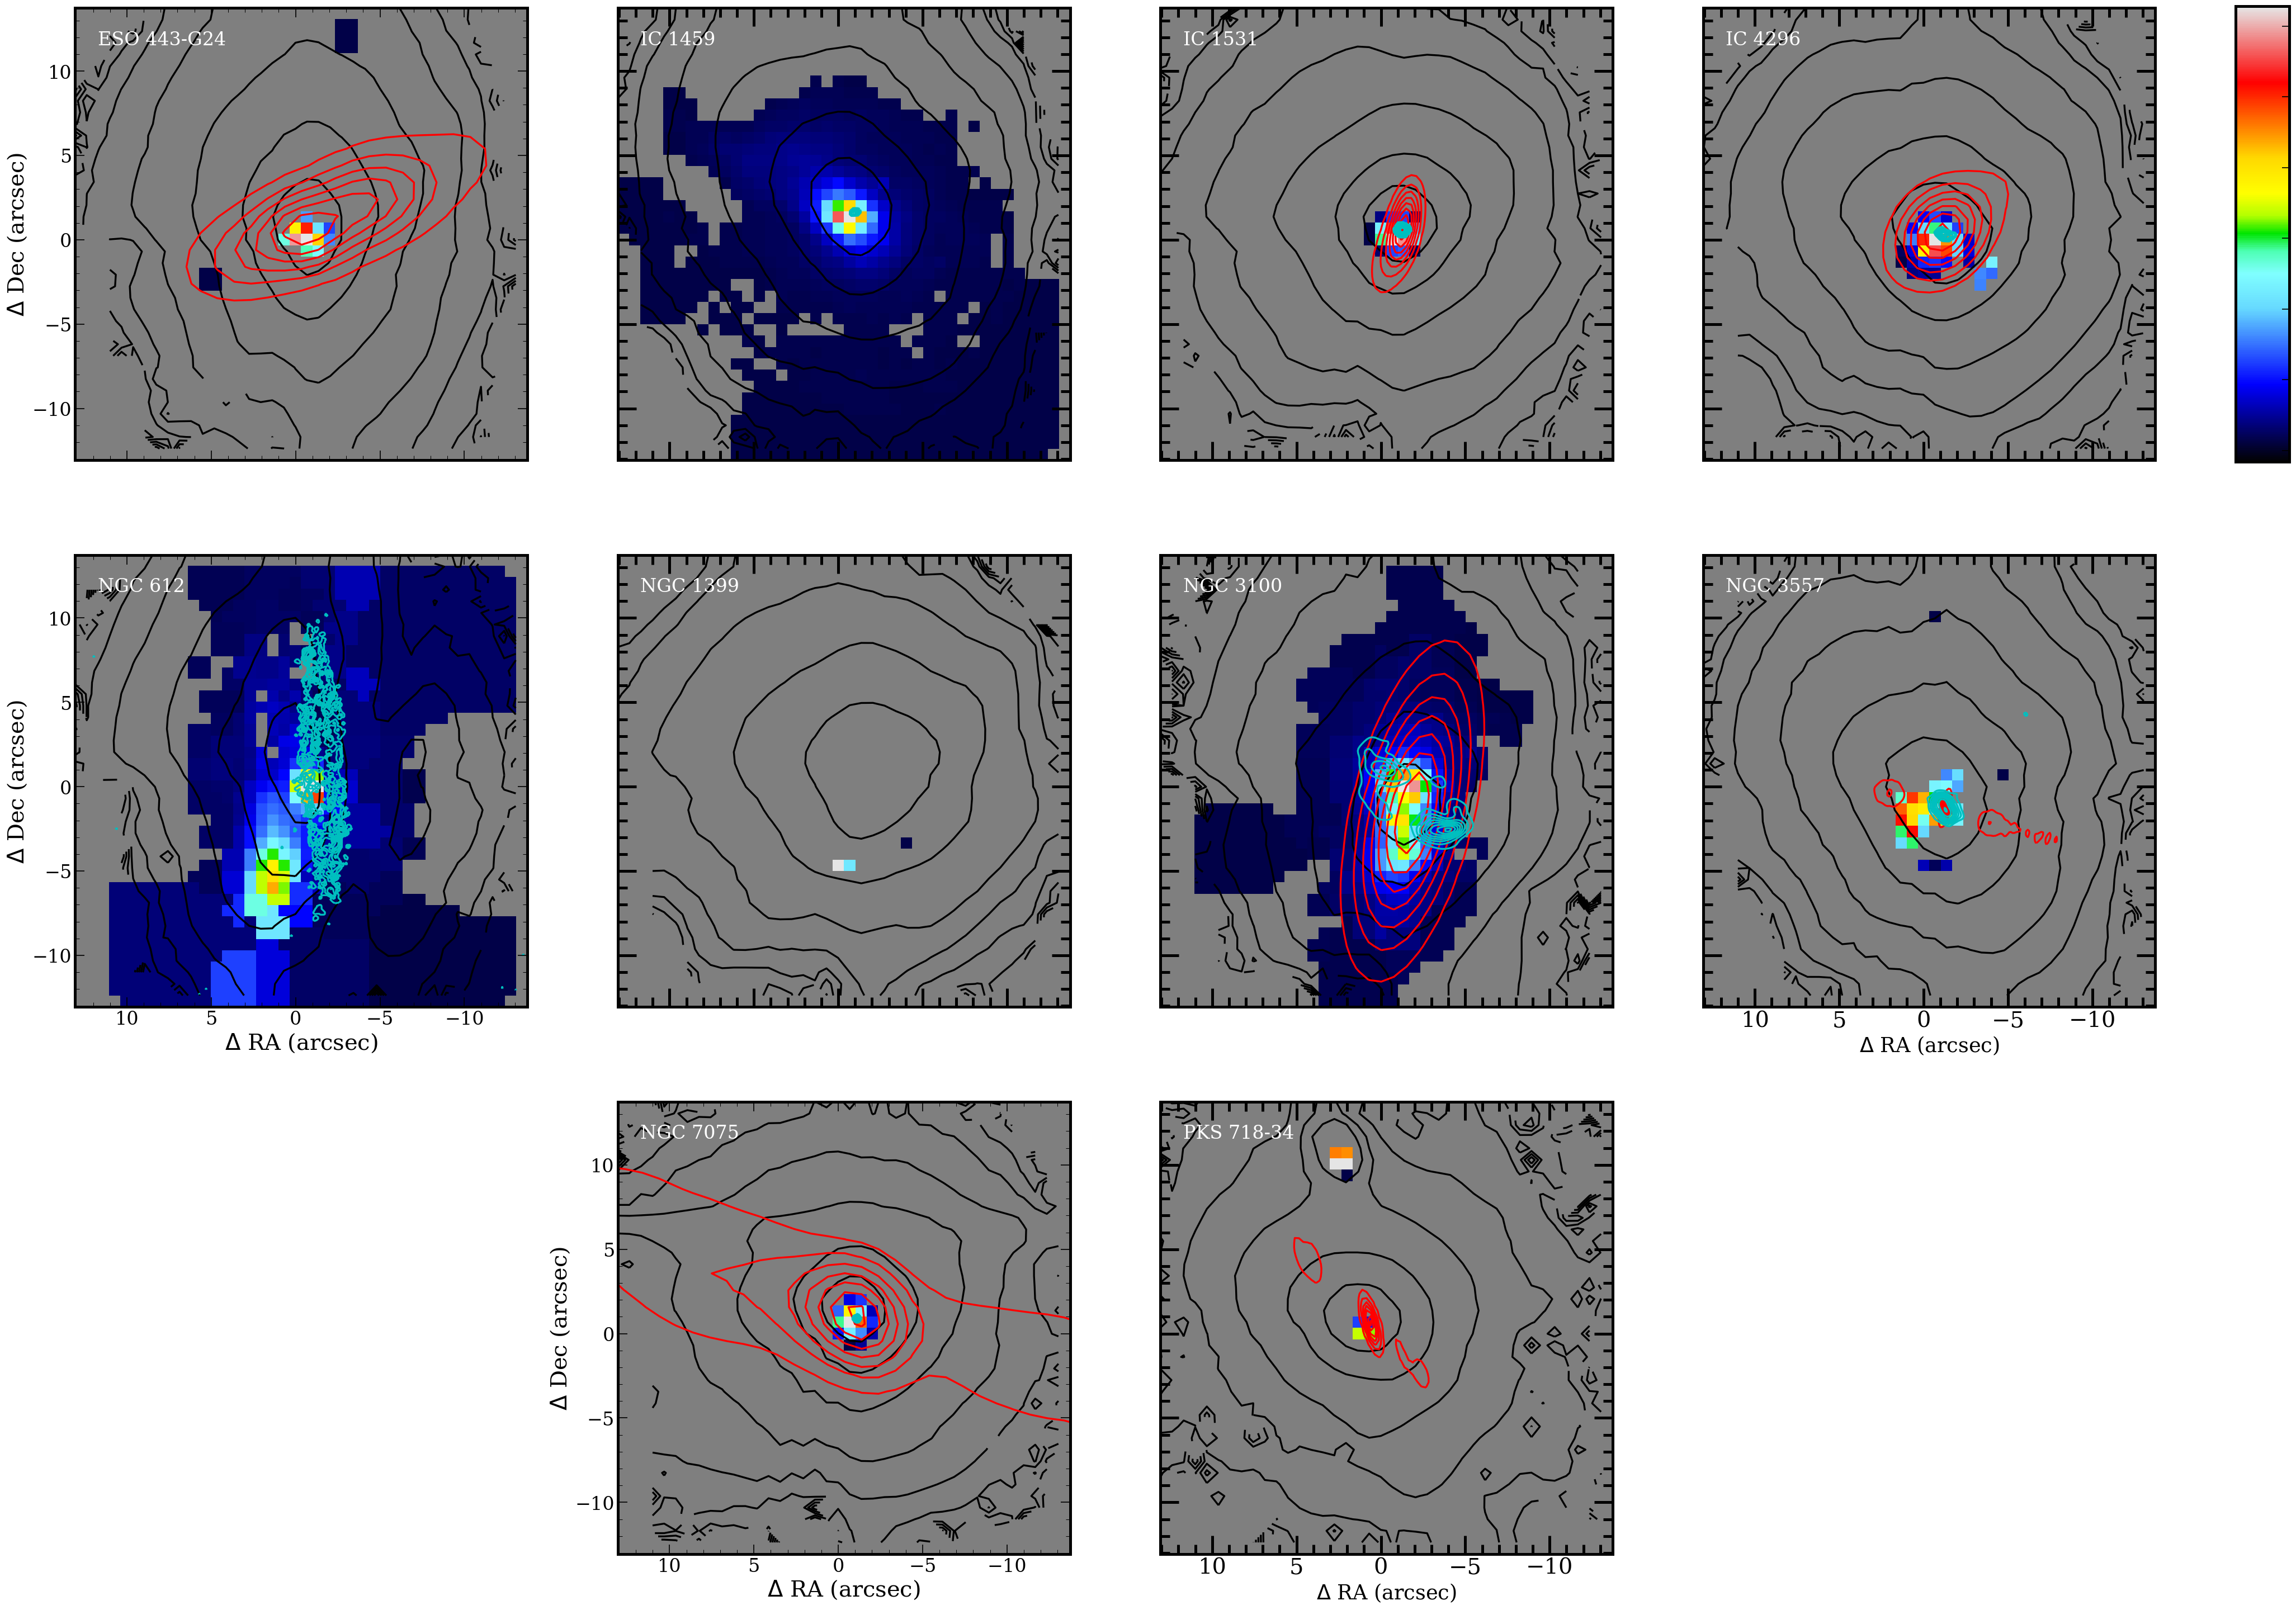
\includegraphics[width=\textwidth]{chapter5/vimos/Hb.png}
			\caption[VIMOS H$\beta$ maps]{VIMOS H$\beta$ maps.} 
			\label{fig:VIMOS_Hb}
		\end{figure}
		\begin{figure}
			\centering
			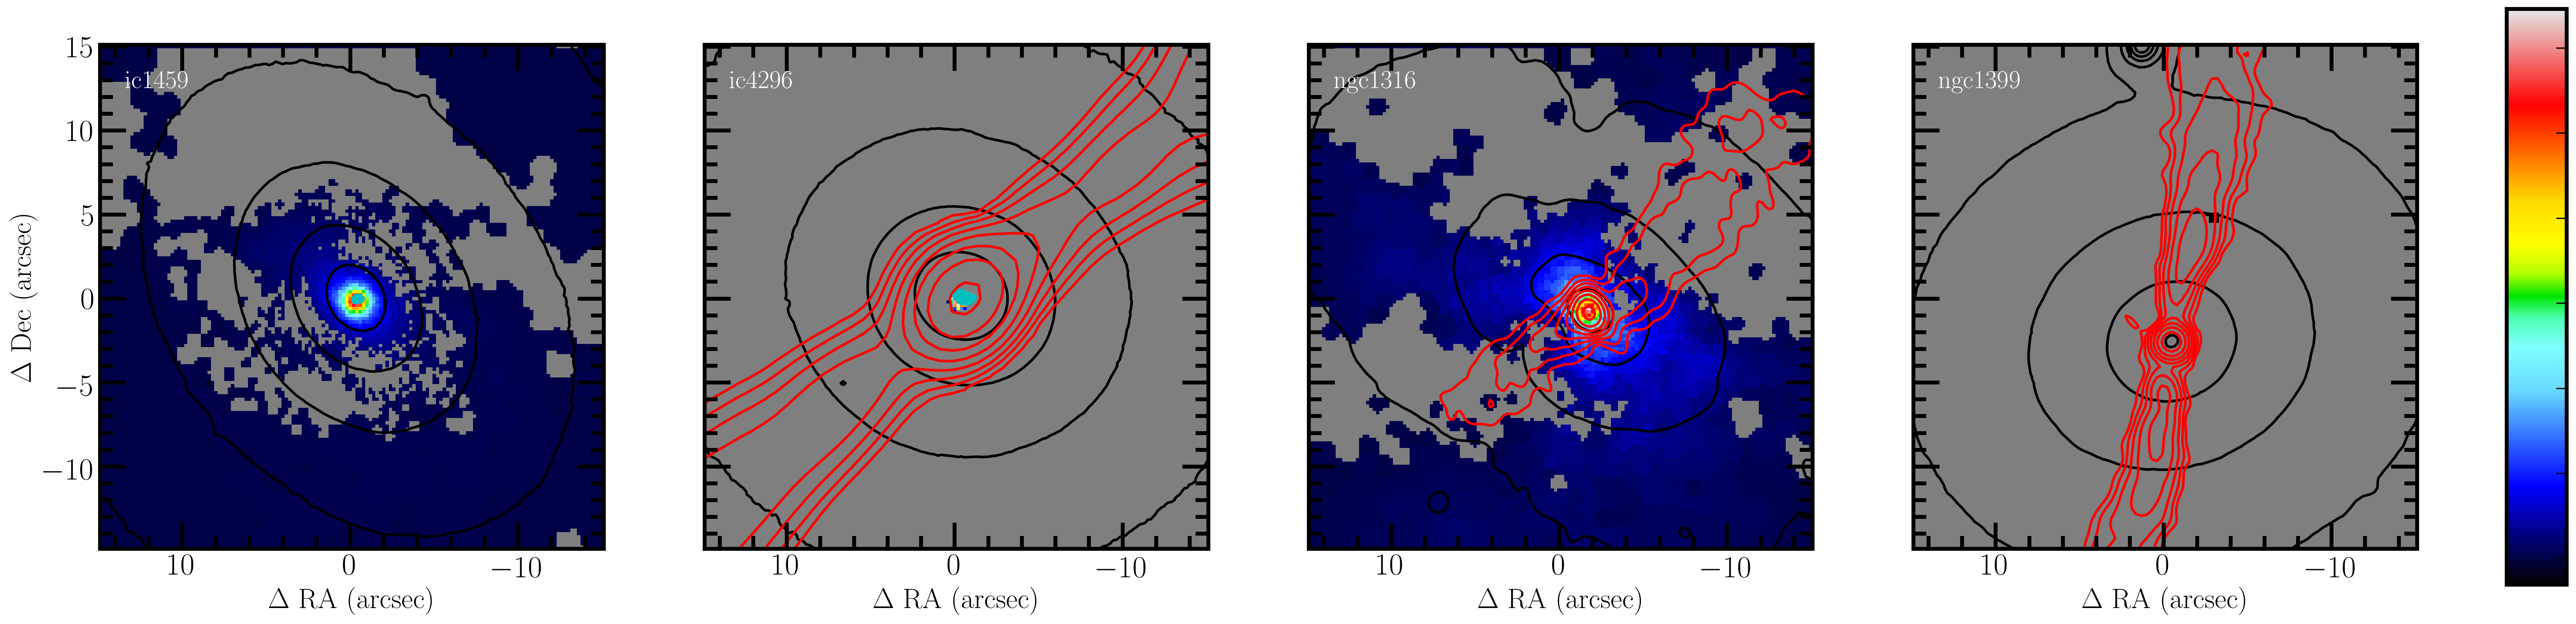
\includegraphics[width=\textwidth]{chapter5/muse/Hb.png}
			\caption[MUSE H$\beta$ maps]{MUSE H$\beta$ maps.} 
			\label{fig:MUSE_Hb}
		\end{figure}


		\begin{figure}
			\centering
			\includegraphics[width=0.4\textwidth]{chapter5/vimos/ngc0612_OIII_flux.png}
			\caption[NGC 612 \bracket{\ion{O}{iii}} image]{NGC 612 [\ion{O}{iii}] map showing a large cloud to the south of the centre of the galaxy, which is not present in the H$\beta$ map (see Fig.\ref{fig:VIMOS_Hb}).} 
			\label{fig:NGC612_OIII}
		\end{figure}


		Because equivalent width is not dependent on overall intensity (except for the initial detection threshold: a line must be detected in order to observe its equivalent width), it can be used to highlight local structures that cannot be seen in flux maps. The equivalent width maps for each emission line for each galaxy in the Southern Sample are shown in Figs.\ref{fig:VIMOS_ew} and \ref{fig:MUSE_ew}. 

		\begin{figure}
			\centering
			\includegraphics[width=\textwidth]{chapter5/vimos/ew.png}
			\caption[VIMOS equivalent width maps]{VIMOS equivalent width maps.} 
			\label{fig:VIMOS_ew}
		\end{figure}
		\begin{figure}
			\centering
			\includegraphics[width=\textwidth]{chapter5/muse/ew.png}
			\caption[MUSE equivalent width maps]{MUSE equivalent width maps.} 
			\label{fig:MUSE_ew}
		\end{figure}

	\subsection{Gas Masses}
		\label{subsec:GasMass}

		Gas masses are derived using the recipe from \citet{Sarzi2005}. This is very rough calculation and the values should not be used for quantitative applications. The approach follows \citet{Kim1989}, and as such
		\begin{equation}
			M_\text{\ion{H}{ii}} = 280 \left(\frac{D}{10\, \mathrm{Mpc}}\right)^2 \frac{F(\mathrm{H\alpha})}{10^{-14} \, \mathrm{erg \, s^{-1} \, cm^{-2}}} \frac{10^3 \, \mathrm{cm^{-3}}}{n_\mathrm{e}} \, ,
		\end{equation}
		where $M_\text{\ion{H}{ii}}$ is the mass in solar mass ($M_\odot$) of \ion{H}{ii} in a galaxy $D$ Mpc away, with an observed H$\alpha$ flux of $F(\mathrm{H\alpha})$. The electron density is assumed to be, $n_\mathrm{e} = 100 \, \mathrm{cm^{-3}}$. 
		% This method assumes B-type recombination and a temperature of 10^4 K.
		Like \citet{Sarzi2005}, we only claim a detection if the amplitude-to-noise ratio (A/N) is $>4$ for [\ion{O}{iii}] and $>2.5$ for H$\beta$. Since most of the gas is centrally concentrated using a large field of view, often only serves to increase the noise (reducing A/N). Our lower limits on the gas mass, are set by the mass measured from the largest aperture that still meets our detection criteria. This would be the gas mass of the galaxy if there was no gas at larger radii. Upper limits are set by the mass found from the H$\alpha$ flux increased by one $\sigma$ for the entire field of view (i.e. $F(\mathrm{H\alpha})+\delta F(\mathrm{H\alpha})$ is used). If a detection is found for the entire field of view, then Table \ref{tab:gasMass} the upper and lower limit columns are combined to show a single value. 


		\begin{table}
			\centering
		\begin{threeparttable}
			\caption{Gas Masses for the Southern Sample.}
			\label{tab:gasMass}
			\begin{tabular*}{0.8\textwidth}{@{\extracolsep{\fill}}l r r r}
				\hline
				\hline
				Galaxy & VIMOS \ion{H}{ii} Mass & MUSE \ion{H}{ii} Mass & Balmer Decrement \\
				& \multicolumn{1}{c}{$[\mathrm{M_odot}]$} & \multicolumn{1}{c}{$[\mathrm{M_odot}]$} & \\
				\hline
				ESO 443-G024 & $5.27 \pm 0.01$ 	& --  		& -- \\
				IC 1459 	& $5.38 \pm 0.01$	&  			&  \\
				IC 1531 	& $5.70 \pm 0.01$	& -- 		& -- \\
				IC 4296		& $5.16 \pm 0.01$	&  			&  \\
				NGC 612 	&  		& -- 		& -- \\
				NGC 1316 	& -- 		&  			&  \\
				NGC 1399 	& $<$ 	&  			&  \\
				NGC 3100 	&  		& -- 		& -- \\
				NGC 3557 	&  		& -- 		& -- \\
				NGC 7075 	&  		& -- 		& -- \\
				PKS 718-34  &  		& -- 		& -- \\
				\hline
				\hline
			\end{tabular*}
			\begin{tablenotes}
			\footnotesize
			\item 
			\end{tablenotes}
		\end{threeparttable}
		\end{table}
		









\section{Ionised Gas Kinematics}
	\label{sec:GasKin}


\section{Sources of Ionising Potential}
	\label{sec:Diagnostics}
	Determining the source of the ionising radiation using line ratio plots, such as Baldwin--Phillips--Terlevich (BPT) diagrams (\citealt{Baldwin1981}; and revised by \citealt{Kewley2001, Kauffmann2003a}), has become increasingly useful tool. That said, there are several important caveats. Firstly, great care must be taken in applying the definitions of each diagnostics line. Much of the literature mis-interprets the classifications. Secondly, in the absence of spatially resolved spectra, low-ionisation nuclear emission-line region (LINER) classifications have often been taken as a marker for jet-mode active galactic nuclei (AGN). As discussed in Section \ref{subsubsection:JetFeedback}, several recent surveys have shown that many of these galaxies may not be bona fide AGN \citep[e.g.][]{Sarzi2005, Sarzi2010, Singh2013, Belfiore2016a}. In such cases, the emission may not even originate from the centre of the galaxies, the location of the supposed AGN. This led to the creation of the low-ionisation emission-line region (LIER) classification, with the same criteria as LINER, but not necessarily in the nuclear region.



